\chapter{Nested Patterns}\indexmain{nested patterns}
\label{cha:nested}

The extension of the rule set language described in the chapter \ref{chaprulelang} by nested patterns in this chapter \ref{cha:nested} and the following chapter \ref{cha:sub} greatly enhances the flexibility and expressiveness of pattern matching and rewriting.
The following patterns to match a simplified abstract syntax tree give a rough picture of the language of nested and subpatterns:
  \begin{example} \label{ex:proggraph}
    \begin{grgen}
test method
{
  m:Method <-- n:Name; // signature of method consisting of name
  iterated { // and 0-n parameters
    m <-- :Variable;
  }  
  
  :AssignmentList(m); // body consisting of a list of assignment statements
}

pattern AssignmentList(prev:Node)
{
  optional { // nothing or a linked assignment and again a list
    prev --> a:Assign; // assignment node 
    a -:target-> v:Variable; // which has a variable as target 
    :Expression(a);  // and an expression which defines the left hand side 
    :AssignmentList(a); // next one, plz
  }
}

pattern Expression(root:Expr)
{
  alternative { // expression may be
    Binary { // a binary expression of an operator and two expresions
      root <-- expr1:Expr;
      :Expression(expr1);
      root <-- expr2:Expr;
      :Expression(expr2);
      root <-- :Operator;
    }
    Unary { // or a unary expression which is a variable (reading it)
      root <-- v:Variable;
    }
  }
}
    \end{grgen}
  \end{example}\label{introexample}


Until now we have seen rules and tests with one left hand side static pattern specification in a direct 1:1 correspondence with its dynamic match in the host graph on a successful application.
From now on we will increase the expressiveness of the pattern language, and dependent on it the rewrite language, to describe much finer and more flexible what patterns to accept.
This will be done by pattern specifications built up from multiple static pattern piece specifications, where the pieces may be matched dynamically zero, one, or multiple times, or are forbidden to exists for the entire pattern to be matched.
These rule set language constructs can be split into nested patterns (negative application condition, positive application condition, nested pattern with cardinality, alternative patterns) and subpatterns (subpattern declaration and subpattern entity declaration, subrule declaration and usage), in this chapter we will focus on the nested patterns:

\begin{rail}  
  NestedPattern: 
    NegativeApplicationCondition |
    PositiveApplicationCondition |
    NestedPatternWithCardinality |
    AlternativePatterns 
    ;
\end{rail}\ixnterm{NestedPattern}


%%%%%%%%%%%%%%%%%%%%%%%%%%%%%%%%%%%%%%%%%%%%%%%%%%%%%%%%%%%%%%%%%%%%%%%%%%%%%%%%%%%%%%%%%%%%%%%%
\section{Negative Application Condition (NAC)}
\indexmain{negative application condition}\indexmainsee{NAC}{negative application condition}\label{nac}

\begin{rail}  
  NegativeApplicationCondition: 
    'negative' lbrace (()+PatternStatement) rbrace;
\end{rail}\ixkeyw{negative}\ixnterm{NegativeApplicationCondition}

With negative application conditions (keyword \texttt{negative}) we can specify graph patterns which forbid the application of a rule if any of them is present in the host graph (cf.~\cite{adam}). 
NACs possess a \indexed{scope} of their own, i.e. names defined within a NAC do not exist outside the NAC. 
Identifiers from surrounding scopes must not be redefined.
If they are not explicitly mentioned, the NAC gets matched independent from them, i.e. elements inside a negative are \texttt{hom(everything from the outside)} by default.
But referencing the element from the outside within the negative pattern causes it to get matched isomorphically/distinct to the other elements in the negative pattern. 
This is a bit unintuitive if you think of extending the pattern by negative elements, but cleaner and more powerful: 
just think of NACs to simply specify a pattern which should not be in the graph, with the possibility of forcing elements to be the same as in the enclosing pattern by name equality.

  \begin{example}
    We specify a variable which is not badly typed, i.e. a node \texttt{x} of type \texttt{Variable} which must not be target of an edge of type \text{type} with a source node of type \texttt{BadType}:
    \begin{grgen}
  x:Variable;
  negative {
    x <-:type- :BadType;
  }
    \end{grgen}
  \end{example}
 
Because NACs have their ``own'' binding, using NACs leads to specifications which might look a bit redundant.

  \begin{example}
    Let's check the singleton condition, meaning there's exactly one node of the type to check, for the type \texttt{RootNamespace}.
    The following specification is \emph{wrong} (it will never return a match):
    \begin{grgen}
  x:RootNamespace;
  negative {
    y:RootNamespace;
  }
    \end{grgen}
	
    Instead we have to specify the \emph{complete} forbidden pattern inside the NAC. This is done by:
    
	\begin{grgen}
  x:RootNamespace;
  negative {
    x;
    y:RootNamespace; // now it is ensured that y must be different from x
  }
    \end{grgen}
	
	Btw: the \texttt{x;} is not a special construct, it's a normal graphlet (cf. \ref{sct:graphlets}).
	
  \end{example} 

If there are several patterns which should not occur, use several negatives.
If there are exceptions to the forbidden pattern, use nested negatives.
As a straight-forward generalization of negatives within positive patterns, negatives may get nested to an arbitrary depth.
Matching of the nested negative pattern causes the matching of the nesting pattern to fail.

\begin{example}
  A fabricated example using parallel as well as nested \texttt{negative}s:
  \begin{grgen}
test onlyOneChildOrAllChildrenHaveExactlyOneCommonChild
{
  root:Class;
  negative {
    root -:extending-> :Class; // root does not extend another class
  }
  root <-:extending- c1:Class; // a class c1 extends root
  negative {
    c1;
    root <-:extending- c2:Class; // there is no c2 which extends root
    negative {
      c1 <-:extending- child:Class -:extending-> c2; // except c1 and c2 have a common child
      negative { // and c1 has no further children
        child;
        c1 <-:extending- :Class;
      }
      negative { // and c2 has no further children
        child;
        c2 <-:extending- :Class; 
      }
    }
  }
}
  \end{grgen}
\end{example}

%negative pattern elements get matched independent from the subpatterns utilizing them
%(explicit patternpath/pattern statement in the negative/independent needed for old behaviour)


%%%%%%%%%%%%%%%%%%%%%%%%%%%%%%%%%%%%%%%%%%%%%%%%%%%%%%%%%%%%%%%%%%%%%%%%%%%%%%%%%%%%%%%%%%%%%%%%
\section{Positive Application Condition (PAC)}
\indexmain{positive application condition}\indexmainsee{PAC}{positive application condition} \label{pac}

\begin{rail}  
  PositiveApplicationCondition: 
    'independent' lbrace (()+PatternStatement) rbrace;
\end{rail}\ixkeyw{independent}\ixnterm{PositiveApplicationCondition}

With positive application conditions (keyword \texttt{independent}) we can specify graph patterns which, in contrast to negative application conditions, must be present in the host graph to cause the matching of the enclosing pattern to succeed.
Together with NACs they share the property of opening a \indexed{scope}, with elements being independent from the surrounding scope (i.e. a host graph element can easily get matched to a pattern element and a PAC element with a different name, unless the pattern element is referenced in the PAC). 
They are used to improve the logical structure of rules by separating a pure condition from the main pattern of the rule amenable to rewriting.
They are used when all matches of a pattern are wanted, and a part of that pattern is available in the graph multiple times, but should not cause combinatorially additional matches; then the \texttt{independent} can be used to check only for the existence of that part, limiting the all-matching to the core pattern.
They are really needed if subpatterns want to match elements which were already matched during the subpattern derivation.

\begin{example}
  A further fabricated example rather giving the intention using \texttt{independent} patterns to check some conditions with only the main pattern available to rewriting:

  \begin{grgen}
rule moveMethod
{
  c:Class --> m:Method;
  csub -:extending-> c;
  csub:Class -e:Edge-> msub:Method;
  
  independent {
    // a complicated pattern to find out that m and msub have same signatures
  }
  independent {
    // a complicated pattern to find out that msub is only using variables available in c
  }
  independent {
    // a complicated pattern to find out that m is not used
  }
 
  modify { // move method upwards
    delete(m);
    delete(e);
    c --> msub;
  }
}
  \end{grgen}
\end{example}

  
%%%%%%%%%%%%%%%%%%%%%%%%%%%%%%%%%%%%%%%%%%%%%%%%%%%%%%%%%%%%%%%%%%%%%%%%%%%%%%%%%%%%%%%%%%%%%%%%
\section{Pattern Cardinality (iterated / multiple / optional)}
\indexmainsee{cardinality}{pattern cardinality}\indexmain{pattern cardinality}\label{cardinality}

\begin{rail}  
  NestedPatternWithCardinality: 
    ('iterated' | 'multiple' | 'optional') lbrace NestedBody rbrace;
  NestedBody: (PatternStatement+) NestedRewriting?;
\end{rail}\ixkeyw{iterated}\ixkeyw{multiple}\ixkeyw{optional}\ixnterm{NestedPatternWithCardinality}

The \indexmain{pattern cardinality} blocks allow to specify how often the nested pattern -- opening a scope -- is to be matched.
Matching will be carried out eagerly, i.e. if the construct is not limiting the number of matches and a further match is possible it will be done.
(The nested body will be explained in Section~\ref{sec:nestedrewrite}.)

\subsection*{The Iterated Block} 
The iterated block is matching the contained subpattern as often as possible, succeeding even in the case the contained pattern is not available (thus it will never fail).
It was included in the language to allow for matching breadth-splitting structures, as in capturing all methods of a class in a program graph.

\begin{example}
  \begin{grgen}
test methods
{
  c:Class;
  iterated {
    c --> m:Method;
  }  
}
  \end{grgen}
\end{example}

\subsection*{The Multiple Block}
The multiple block is working like the iterated block, but expects the contained subpattern to be available at least once; if it is not, matching of the multiple block and thus its enclosing pattern fails.

\begin{example}
  \begin{grgen}
test oneOrMoreMethods
{
  c:Class;
  multiple {
    c --> m:Method;
  }
}
  \end{grgen}
\end{example}

\subsection*{The Optional Block}
The optional block is working like the iterated block, but matches the contained subpattern at most once; further occurrences of the subpattern are left unmatched.
If the nested pattern is available, it will get matched, otherwise it won't; matching of the optional block will succeed either way.

\begin{example}
  \begin{grgen}
test variableMaybeInitialized
{
  v:Variable; // match variable
  optional { // and an initialization with a different one if available
    v <-- otherV:Variable;
  }
}
  \end{grgen}
\end{example}

\subsection*{Iteration Breaking} 
If an application condition inside an iteration block fails, then that potential match of the iterated pattern is thrown away and matching continues trying to find further matches.
Sometimes a different behaviour is wanted, with an application condition terminating the iteration and causing it to fail.
This would allow to check with a single rule that "every pattern X must also satisfy Y" holds.
This behaviour is supported with the \indexmain{break}\texttt{break} keyword prepended to an application condition, transforming it into an iteration breaking condition.

\begin{example}
If the \texttt{negative} matches, not only the current iteration instance is prevented from matching, but the entire \texttt{iterated} (and thus the \texttt{test}) is failing to match:
  \begin{grgen}
test forEachXMustNotBeTheCaseY
{
  iterated {
    <X>;
    break negative { 
      <Y>;
    }
  }
}
  \end{grgen}

If the \texttt{independent} does not match, not only the current iteration instance is prevented from matching, but the entire \texttt{iterated} (and thus the \texttt{test}) is failing to match:
  \begin{grgen}
test forEachXMustBeTheCaseY
{
  iterated {
    <X>;
    break independent { 
      <Y>;
    }
  }
}
  \end{grgen}
\end{example}

\begin{warning}
Pattern cardinality constructs are match/rewrite-all enumeration blockers.
For every pattern instance, the iterated/... yields only one match, even if in all mode (used in/from all-bracketed rules).
\end{warning} 


%%%%%%%%%%%%%%%%%%%%%%%%%%%%%%%%%%%%%%%%%%%%%%%%%%%%%%%%%%%%%%%%%%%%%%%%%%%%%%%%%%%%%%%%%%%%%%%%
\section{Alternative Patterns}
\indexmain{alternative patterns}\label{alternative}

\begin{rail}  
  AlternativePatterns: 
    'alternative' lbrace ((CaseName lbrace NestedBody rbrace)+()) rbrace;
\end{rail}\ixkeyw{alternative}\ixnterm{AlternativePattern}

With the alternative block you can specify several nested alternative patterns. One of them must get matched for the matching of the alternative (and thus its directly nesting pattern) to succeed, and only one of them is matched per match of the alternative / overall pattern.
The order of matching the alternative patterns is unspecified, especially it is not guaranteed that a case gets matched before the case textually following -- if you want to ensure that a case cannot get matched if another case could be matched, you must explicitly prevent that from happening by adding negatives to the cases.
In contrast to the iterated which locally matches everything available and inserts this combined match into the current match, the alternative decides for one case match which it inserts into the current match tree, ignoring other possible matches by other cases. 

\begin{example}
  \begin{grgen}
test feature(c:Class)
{
  alternative // a feature of the class is either
  {
    FeatureMethod { // a method
      c --> :Method;
    }
    FeatureVariable { // or a variable
      c --> :Variable;
    }
    FeatureConstant { // or a constant
      c ---> :Constant;
    }
  }
}  
  \end{grgen}
\end{example}

\begin{example}
  \begin{grgen}
test variableMaybeInitialized
{
  v:Variable; // match variable
  alternative { // and an initialization with a different one if available
    Empty {
      // the empty pattern matches always
      negative { // so prevent it to match if initialization is available
        v <-- otherV:Variable;
      }
    }
    Initialized { // initialization
      v <-- otherV:Variable;
    }
  }
}
  \end{grgen}
\end{example}

\begin{example} \label{ex:retypelhs}
When working with the subtyping hierarchy one may be interested in matching in a first step an abstract base class,
specifying the rewriting behaviour for this base class once,
and in a refinement step in an alternative the different possible subtypes, 
then being able to access their specific attributes and being able of giving different additional rewrite parts.
	\begin{grgen}
test refineFeature
{
  f:Feature; // match abstract base class Feature

  alternative {
    Variable {
      v:Variable<f>; // try to cast to concrete Variable, if succeeds we can access the Variable attributes
    }
    Method {
      m:Method<f>; // try to cast to a concrete Method, if succeeds we can access the Method attributes
    }
  }
  
  modify {
    // do stuff common to a Feature here
  }
}
	\end{grgen}
\end{example}


\begin{example}

\begin{center}
  \parbox{0.99\linewidth}{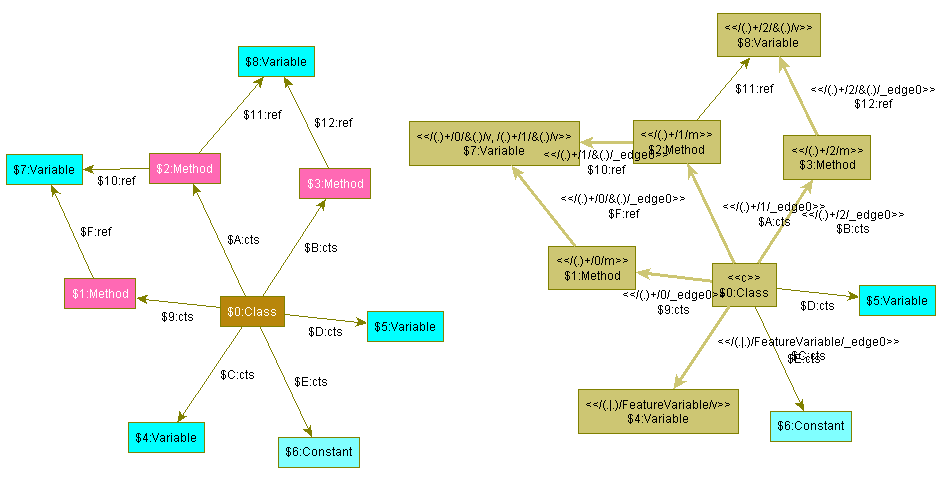
\includegraphics[width=\linewidth]{fig/exnested}}
\end{center}

The image from above shows an example how a structure is matched by several pieces.
At the left, the plain host graph, at the right with the match of \texttt{classWithStuff} inscribed.

\begin{grgen}
test classWithStuff
{
  c:Class; // get a class
	
  multiple { // get all of its methods, expect at least one
    c --> m:Method;
		independent { // expect an argument variable
		  m -:ref-> v:Variable;
		}
  }	

  alternative // additionally, match one of either
  {
    FeatureVariable { // a variable
      c --> v:Variable;
    }
    FeatureConstant { // or a constant
      c --> ct:Constant;
    }
  }
}
\end{grgen}

The example matches a class node \texttt{c} and its contained methods with a \texttt{multiple} pattern -- note the 3 instances of the pattern in the host graph getting captured by the single pattern description
(\verb#/(.)+/1/m# reads as multiple pattern (see Table~\ref{keywordregexpsyntax} explaining the regular expression syntax), match instance \texttt{1} (starting at \texttt{0}), pattern element \texttt{m}.)

Additionally, one of the alternative cases of a variable or a constant is matched -- here we got two potential patterns, from which only one is matched, capturing node \verb#$4# out of the potential targets \verb#$4#, \verb#$5#, \verb#$6#
(\verb#/(.|.)/FeatureVariable/v# reads as alternative, case \texttt{FeatureVariable}, pattern element \texttt{v}.)

The independent that is used to reference a parameter variable \texttt{v} from method \texttt{m} allows to re-match an already matched variable that would be otherwise shut out from getting matched again
(happened here with node \verb#$7#, matched from instances $0$ and $1$ of the multiple pattern; a graph element is annotated with all matching pattern elements).

\end{example}



%%%%%%%%%%%%%%%%%%%%%%%%%%%%%%%%%%%%%%%%%%%%%%%%%%%%%%%%%%%%%%%%%%%%%%%%%%%%%%%%%%%%%%%%%%%%%%%%
\section{Nested Pattern Rewriting}
\indexmain{nested pattern rewrite}\label{sec:nestedrewrite}

Until now we focused on the pattern matching of nested and subpatterns -- but we're not only interested in finding patterns combined from several pattern pieces, we want to rewrite the pattern pieces, too.
So we will extend the language of the structure parser introduced so far into a language for a structure transducer.
This does not hold for the application conditions, which are pure conditions, but for all the other language constructs introduced in this chapter.

\begin{rail}  
  NestedRewriting: ('replace' | 'modify') lbrace (()+RewriteStatement) rbrace;
\end{rail}\ixnterm{NestedRewriting}\ixkeyw{replace}\ixkeyw{modify}

Syntactically the rewrite is specified by a modify or replace clause nested directly within the scope of each nested pattern;
in addition to the rewrite clause nested within the top level pattern.
Semantically for every instance of a pattern piece matched its dependent rewrite is applied. 
So in the same manner the complete pattern is assembled from pattern pieces, the complete rewrite gets assembled from rewrite pieces
(or operationally: rewriting is done along the match tree by rewriting one pattern piece after the other).
Note that \texttt{return} statements are not available as in the top level rewrite part of a rule, and the \texttt{exec} statements are slightly different.

For a static pattern specification like the iterated block yielding dynamically a combined match of zero to many pattern matches, every submatch is rewritten, according to the rewrite specification applied to the host graph elements of the match bound to the pattern elements
(if the pattern was matched zero times, no dependent rewrite will be triggered - but note that zero matches still means success for an iterated, so the dependent rewrite piece of the enclosing pattern will be applied).
This allows e.g. for reversing all edges in the iterated-example (denoting containment in the class), as it is shown in the first of the following two examples.
For the alternative construct the rewrite is specified directly at every nested pattern, i.e. alternative case as shown in the second of the following two examples); the rewrite of the matched case will be applied.

Nodes and edges from the pattern containing the nested pattern containing the nested rewrite are only available for deletion or retyping inside the nested rewrite if it can be statically determined this is unambiguous, i.e. only happening once.
So only the rewrites of alternative cases, optional patterns or subpatterns may contain deletions or retypings of elements not declared in their pattern (in contrast to iterated and multiple pattern rewrites).

\begin{example}
%This is an example for a rewrite part nested within an iterated block. - without the comment the two examples fit on one page
  \begin{grgen}
rule methods
{
  c:Class;
  iterated {
    c --> m:Method;

    replace {
      c <-- m;
    }
  } 

  replace {
    c;
  }  
}
  \end{grgen}
\end{example}

\begin{example}
%This is an example for a rewrite parts nested within alternative cases. - without the comment the two examples fit on one page
  \begin{grgen}
rule methodWithTwoOrThreeParameters(m:Method)
{
  alternative {
    Two {
      m <-- n:Name;
      m <-e1:Edge- v1:Variable;
      m <-e2:Edge- v2:Variable;
      negative {
        v1; v2; m <-- :Variable;
      }

      modify {
        delete(e1); m --> v1;
        delete(e2); m --> v2;	    
      }
    }
    Three {
      m <-- n:Name;
      m <-e1:Edge- v1:Variable;
      m <-e2:Edge- v2:Variable;
      m <-e3:Edge- v3:Variable;

      modify {
        delete(e1); m --> v1;
        delete(e2); m --> v2;
        delete(e3); m --> v3;
      }
    }

  //modify { can be omitted - see below
  //}
}
  \end{grgen}
\end{example}

\begin{note} \label{omitmodify}
In case you got a \texttt{rule} or \texttt{pattern} with an empty \texttt{modify} clause, with all the real work going on in an \texttt{alternative} or an \texttt{iterated}, you can omit the empty \texttt{modify} clause.
This is a small syntactic convenience reducing noise which is strictly restricted to the top level pattern --- omitting rewrite parts of nested patterns specifies the entire pattern to be match-only (like a \texttt{test}; this must be consistent for all nested patterns).
\end{note}

\begin{example}
This is an example which shows how to decide with an alternative on the target type of a retyping depending on the context.
Please note the omitted rewrite (cf. \ref{omitmodify}).

  \begin{grgen}
rule alternativeRelabeling
{
  m:Method;
  
  alternative {
    private {
      if { m.access == Access::private; }

      modify {
        pm:PrivateMethod<m>;
      }
    }
    static {
      negative {
        m <-- c;
      }

      modify {
        sm:StaticMethod<m>;
      }
    }
  } 
}
  \end{grgen}
\end{example}
